\chapter{North Sea Data Collection} \label{ch:NDD}

At this stage, the automatic photo-identification system in development is capable of detecting cetaceans in large panoramic images and post-processing these detections into a form ready for individual identification, as outlined in Chapter \ref{ch:cetDet}. So far, the detector has been trained and tested on data collected by Newcastle University's Marine MEGAfauna Lab whilst researching the abundance of Indo-Pacific bottlenose dolphins (\textit{Tursiops aduncus}) off the coast of Zanzibar, Tanzania \cite{sharpe_indian_2019}. 

Whilst the Marine MEGAfauna Lab research heavily in the Indian Ocean around Zanzibar \cite{yang_description_2020, temple_life-history_2020, temple_marine_2019, temple_marine_2018, weigmann_revision_2020, barrowclift_social_2017}, this is not the only place they operate \cite{temple_by-catch_2021, yang_classification_2017, yang_influence_2022}. In recent years, their work has begun to include more local waters such as the North Sea off the coast of Northumberland, UK \cite{van_bressem_visual_2018, yang_characterization_2021}. These waters are known to host a wide variety of marine mammals, with the Marine MEGAfauna Lab focussing efforts specifically on the bottlenose dolphin (\textit{Tursiops truncatus}) and white-beaked dolphin (\textit{Lagenorhynchus albirostris}) populations. 

Near the end of the Mask-RCNN detection model's completion, the Marine MEGAfauna Lab were preparing to begin a large scale bottlenose and white-beaked abundance estimate and health assessment survey. As such the opportunity arose to validate the detector's generalisability on data which is similar in composition and purpose, however was collected in a different geographic location, at a different time, and containing different species to the data used to train and test the detector.

As a result, this Chapter discusses the collection of abundance estimate data in Northumberland, UK for the purpose of model and technique evaluation as outlined in Chapter \ref{ch:cetDet}. In order to achieve this evaluation, the photo-identification data was curated and transformed from a biological catalogue into a computer vision dataset known as The Northumberland Dolphin Dataset 2020 (NDD20) - the creation of which will also be discussed. 

\section{Data Collection}\label{ch:NDD,sec:dataCollection}

The following Section provides context for the data collection survey, beginning by briefly outlining the geographic area in which the data was collected and discussion of why the area was chosen. Next the survey effort is discussed in detail, including a run-down of the methodology used, for the purposes of reproducibility. 

\subsection{The Survey Area}\label{ch:NDD,sec:dataCollection,sub:surveyArea}

Data collection was conducted in and around the Coquet to St. Mary's Marine Conservation Zone (MCZ), located off the coast of Northumberland, UK. The MCZ, established in January 2016 through powers granted by the Marine and Coastal Access Act 2009 \cite{noauthor_marine_2009}, covers approximately 40km of coastline from Almouth in the north to Whitley Bay in the south, extending outwards 7.5km at its greatest to cover an area around 192km$^{2}$. A map of the survey area and MCZ can be seen in Figure \ref{fig:survey-map}.

 \begin{figure}
	\begin{center}
		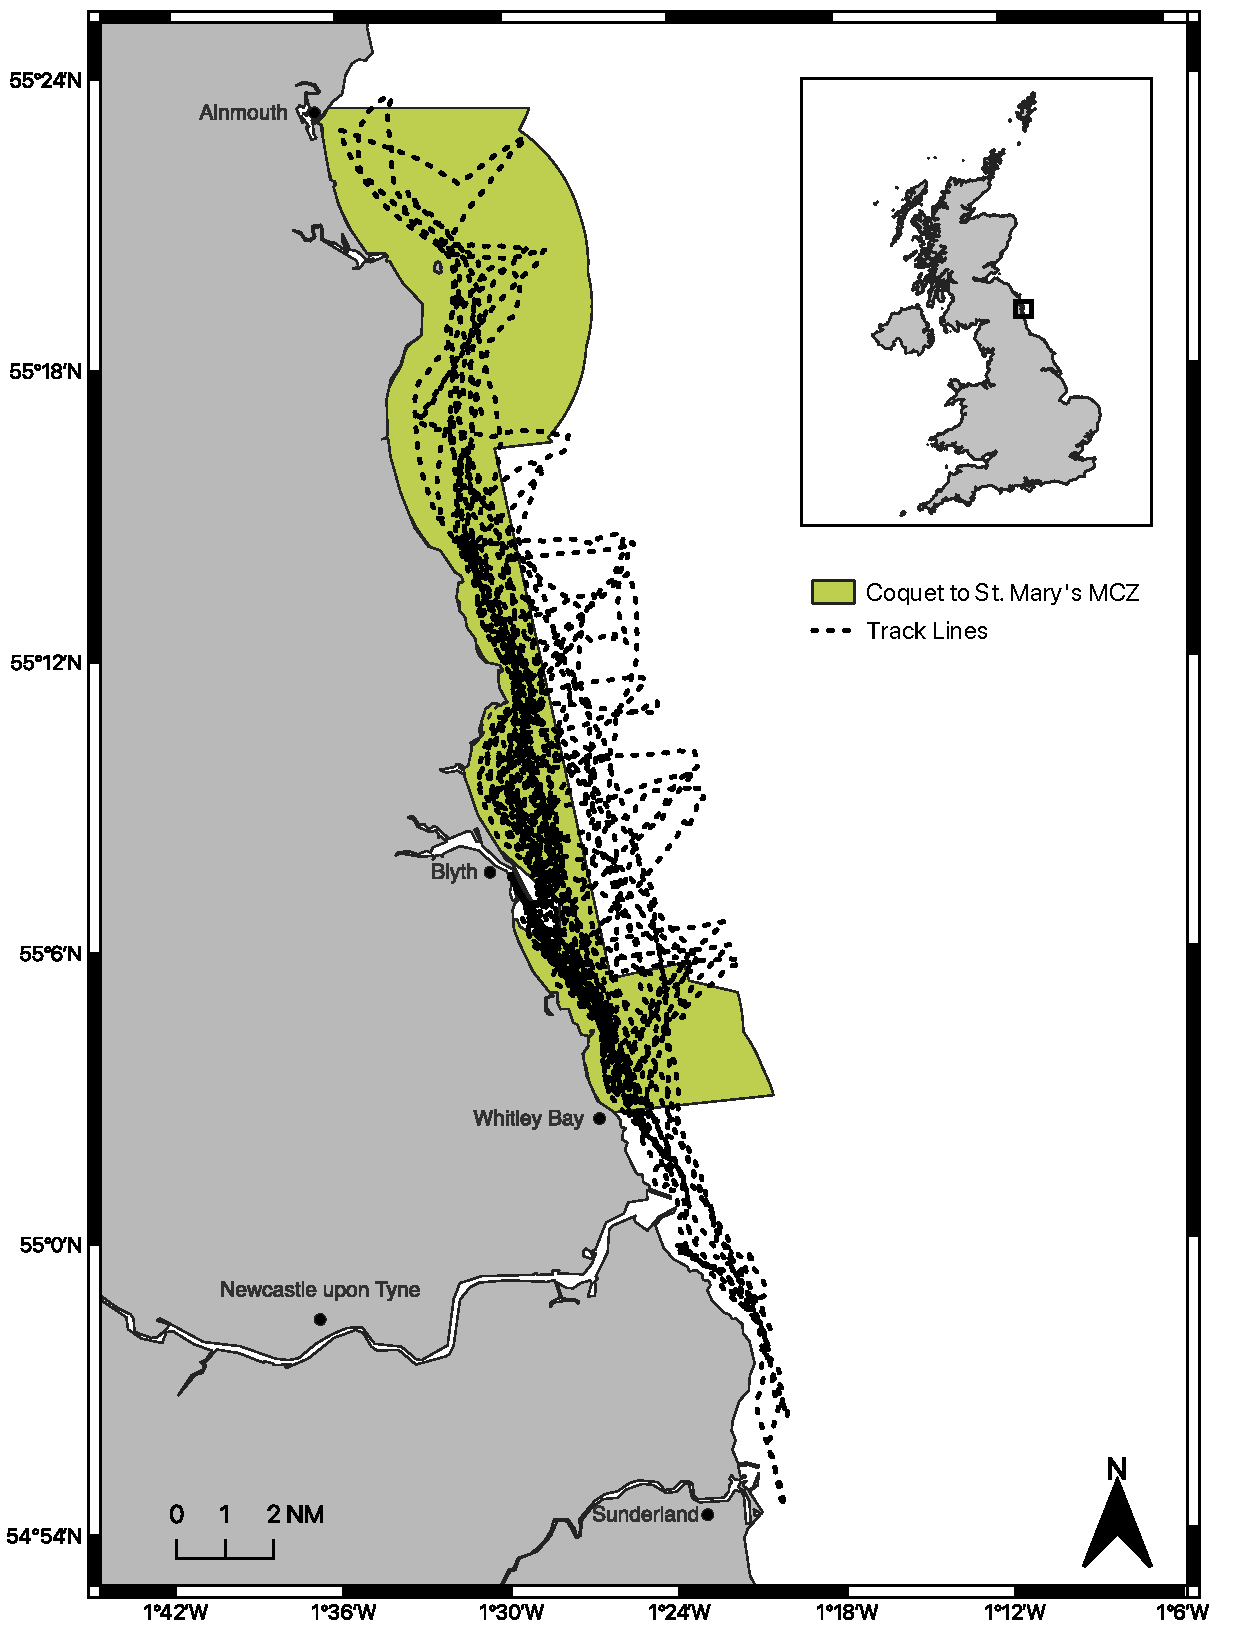
\includegraphics[scale=0.7]{Chapter4/figs/survey_map.pdf}
	\end{center}
	\caption{Map of the survey area, with the Coquet to St. Mary's MCZ highlighted. Track lines for all survey days are overlaid.}
	\label{fig:survey-map}
\end{figure}

The area is of high importance, supporting a wide variety of marine life thanks to sections of intertidal and sub-tidal rock and sediment, making it fertile feeding grounds for the bottlenose and white-beaked dolphins which make use of the area. As a result of this fertility, as well as waters up to 30m deep in some places, the MCZ sees high levels of fishing activity - typically for crustaceans using pots \cite{stephenson_spatial_2017}. Whilst these fishing vessels operate from a number of small ports throughout the North East of England, the MCZ itself lies close to the large Port of Blyth. As a result, the MCZ boundary provides a 250m buffer zone around the limits of the port in order to reduce economic damage. This survey region was selected as no previous surveying had been undertaken in the area for the purposes of cetacean abundance estimates and health assessment.

\subsection{Survey Effort}\label{ch:NDD,sec:dataCollection,sub:surveyEffort}

Dedicated bottlenose and white-beaked dolphin photo-identification surveys were conducted in the MCZ between 19/07/2019 and 10/10/2019, with a total of 27 surveys undertaken. These were performed using a 5.6m rigid inflatable boat (RIB) with a 50 horsepower four-stroke outboard engine. All surveys began from Newcastle University's Blyth Marine Station, located in the Port of Blyth, before entering the MCZ.

Surveys initially began by following set transect lines, traversing between the northern and southern-most points of the MCZ. Thanks to limited success encountering individuals strictly following transect lines however, the survey switched to more opportunistic surveying based on reports from two citizen science groups: the Newbiggin-by-the-Sea Dolphin Watch\footnote{Newbiggin-by-the-Sea Dolphin Watch: \href{https://en-gb.facebook.com/groups/NEWILDDOLPHINMONITORINGPROJECT/}{facebook.com/groups/NEWILDDOLPHINMONITORINGPROJECT}} and the North East Cetacean Project\footnote{North East Cetacean Project: \href{https://en-gb.facebook.com/groups/NorthEastCetaceanProject/about/}{facebook.com/groups/NorthEastCetaceanProject}}. The use of citizen scientists for photo-id surveys has seen increased prevalence in recent years, with multiple studies producing promising results if access to groups of dedicated citizen scientists is available, like in Northumberland \cite{araujo_population_2017, currie_conservation_2018, armstrong_photographic_2019, araujo_photo-id_2019}. Track lines showing movement of the vessel were recorded via GPS tracking, and can be seen in Figure \ref{fig:survey-map}. When dolphins were encountered, the time stamp was recorded alongside other effort data such as direction of travel, sea state, species, group size, and demographic composition.

Surveys were only conducted in Beaufort Sea States $\le 3$ \cite{world_meteorologicial_society_beaufort_1970} without heavy rain. Outside of these conditions surveying can become unsafe and the photographs unusable for photo-id because of swell and lens splash. Due to the nature of the North Sea, conditions outside of these restrictions can be common. Surveying was performed using the constant scanning method \cite{mann_behavioral_1999}, with cues including sight of dorsal fins breaching the waterline, splashing, and leaping. For each survey the vessel was manned by at least two dedicated observers and a skipper, in line with other photo-id surveys \cite{sharpe_indian_2019, bessesen_lacaziosis-like_2014, silva_winter_2012}.

Individual dolphins in an encounter were photographed randomly using a Canon EOS 550D Digital SLR with a Canon 70–200mm zoom lens, aiming to capture photographic data for every individual present. Multiple photographs were captured of each cetacean over the course of the encounter to ensure identifiable information could be fully captured. When capturing an encounter care was taken not to approach individual cetaceans at an angle less than $30^{\circ}$, keeping as parallel as possible and to speeds no greater than 6 knots in order to prevent the cetaceans becoming stressed or injured as per Marine Management Organisation guidelines. All members of the survey team were trained in minimising wildlife disturbance through the WiSe Scheme by the Yorkshire Wildlife Trust\footnote{WiSe Scheme: \href{https://www.wisescheme.org/}{wisescheme.org}}, with the survey itself having the approval of Newcastle University's Ethics Board.

\subsection{Field Season Summary}\label{ch:NDD,sec:dataCollection,sub:summary}

Of the 27 days where surveys were conducted 14 contained encounters. Of these, 12 were made up of bottlenose dolphin; only two were made up of white-beaked dolphin. No encounters contained both species. Groups were defined using the 10m chain rule \cite{smolker_sex_1992}. Group size averaged 12 for bottlenose dolphins, typical for the species \cite{shane_ecology_1986}. Altogether 40 individuals were identified and catalogued, broken down into 30 bottlenose and 10 white-beaked dolphins. Of all animals encountered, 27\% were calves. They have been excluded from this analysis as they could not be considered independent due to reliance on their mothers, and had not yet developed permanent markings.

Images collected were processed for use in the photo-identification catalogue as to remove any images with no value, such as those which were out of focus or did not contain any cetacean. Animals present in the images were coded according to their distinctiveness as per the guidelines presented in \cite{urian_recommendations_2015}. Those coded D1 were considered very distinctive with little chance of misidentification, whilst those coded D2 were considered moderately distinctive with small prominent markings which could allow for a high chance of correct classification provided the image is clear. CF coded individuals were those which contained little to no identifying information which have a high chance of misclassification. Once coded, animals considered D1 and D2 were individually identified.

\section{The Northumberland Dolphin Dataset 2020}\label{ch:NDD,sec:NDD20}

The fieldwork season and data processing undertaken resulted in a photo-identification catalogue of bottlenose and white-beaked dolphins currently inhabiting the Coquet to St. Mary's MCZ. Photo-identification catalogues utilised in marine biology however are not in the form required for training or validating a computer vision model. As such, further processing was required to transform the catalogue into a dataset capable of both validating the instance segmentation model developed in Chapter \ref{ch:cetDet}, as well as training a model for fine-grained individual identification. This Section discusses the creation of the Northumberland Dolphin Dataset 2020 (NDD20) \cite{trotter_ndd20_2020}, the computer vision dataset created from the photo-identification catalogue.

\subsection{Above Water Data}\label{ch:NDD,sec:NDD20,sub:aboveWaterData}

During fieldwork 4940 images were collected which contained part of a cetacean above the water line. Of these, 2201 images were considered usable for the creation of NDD20. Issues rending images unusable included a significant amount of water splash obscuring the cetacean, poor lighting conditions, or where individuals in a pod were too close together to accurately determine by eye the outline of all individuals. 

From manual analysis it was determined that not all images contained enough identifying information for individual classification labels. Because of this, the decision was made to include multiple levels of granularity to the dataset. As all images contained part of a cetacean, each one could be labelled to allow for instance segmentation training. To enable this, each mask located was given the label \texttt{dolphin}. Next, masks could be provided a fine-grained species classification. Thanks to the difference in colour between bottlenose and white-beaked dolphins, every mask labelled for instance segmentation could also be provided a species label - either \texttt{BND} or \texttt{WBD} representing bottlenose and white-beaked dolphin respectively. 

At the highest level of granularity, some masks contained enough information to allow for individual identification. If an ID could be attained with high confidence, likely from images with D1 or D2 coded individuals, the mask containing the individual was provided an \texttt{ID} label. To protect ongoing cetacean research efforts a pseudo-anonomisation has been performed. This however does not diminish the value of this data to computer vision researchers. It is not the case that images with sequential filenames were captured sequentially, and all individual IDs have been randomly allocated a numerical value rather than the code given to them by the Marine MEGAfauna Lab. All EXIF data found in the images has also been removed. The photo-identification catalogue itself is not publicly hosted at this time.

Data was labelled at a pixel level using the VGG Image Annotator \cite{dutta_via_2019} in a similar fashion to the Zanzibar dataset as discussed in Section \ref{ch:cetDet,sec:initialTesting,sub:zanzibar}. In order to speed up the process data labellers were employed through Newcastle University's Jobs On Campus service\footnote{Newcastle University Jobs On Campus: \href{https://www.ncl.ac.uk/careers/jobs/opportunities-on-campus/jobsoc/\#jobsocoverview}{ncl.ac.uk/careers/jobs/opportunities-on-campus/jobsoc/}} to manually annotate the masks and label them for instance segmentation. Once complete all masks were checked for error correcting and consistency purposes. Afterwards, the extra labels for both species and individual level identification were added. As this required expert knowledge, data labellers were not utilised for this. Example above water images from NDD20 and the labels assigned can be seen in Figure \ref{fig:above-water-example}.

\begin{figure}
	\begin{center}
		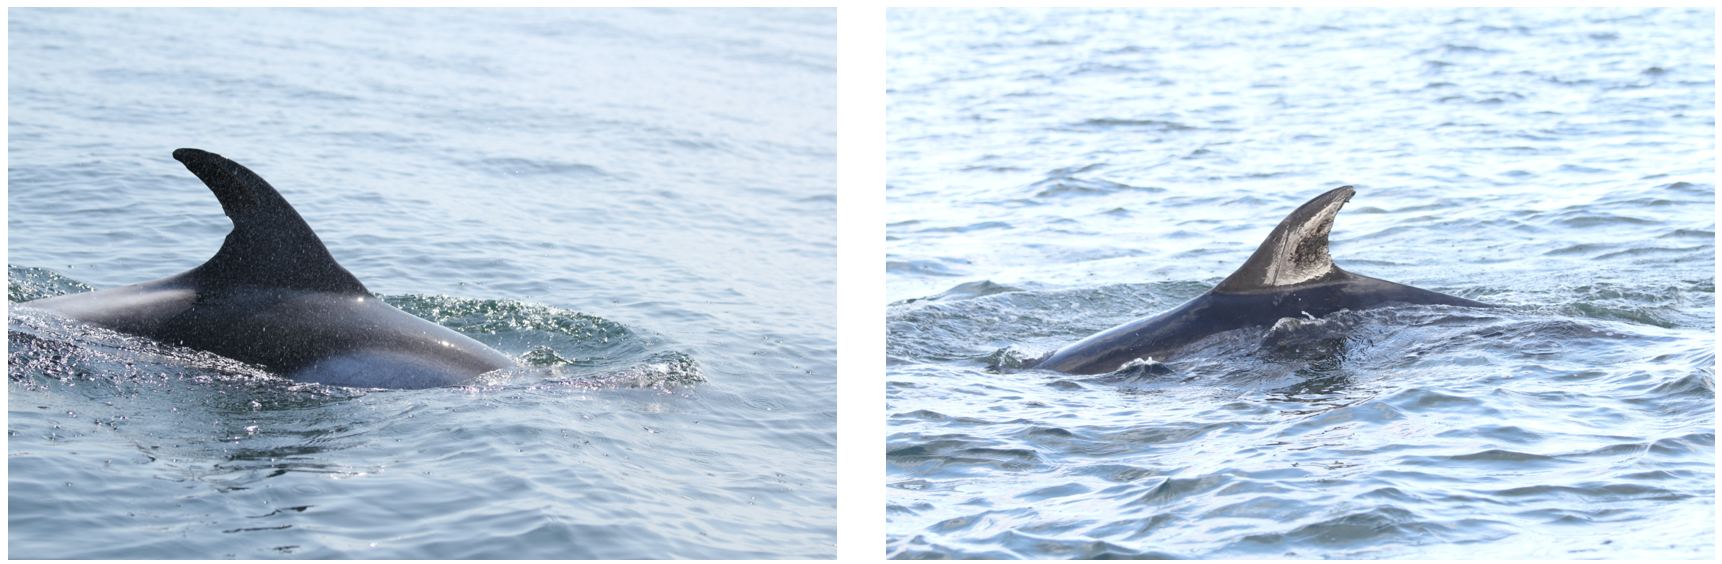
\includegraphics[scale=0.5]{Chapter4/figs/aweg.png}
	\end{center}
	\caption{Example above water images. Both images contain one mask with the following attributes: Left - \texttt{object:dolphin}, \texttt{species:WBD}, \texttt{ID:11}. Right - \texttt{object:dolphin}, \texttt{species:BND}, \texttt{ID:8}.}
	\label{fig:above-water-example}
\end{figure}

\subsection{Below Water Data}\label{ch:NDD,sec:NDD20,sub:belowWaterData}

In addition to the above water imagery captured during fieldwork, NDD20 also contains below water images. Whilst this data has not been utilised in the work on automatic photo-id presented in this thesis it is important to discuss all aspects of the dataset created. Images contained in the below water section of NDD20 are a subset of a much larger collection of images collected by the Marine MEGAfauna Lab during work in the Farnes Deep MCZ, a glacial trench situated approximately 11km from the Northumberland coast. Opportunistic surveys undertaken since 2011 have shown the area to contain a high abundance of white-beaked dolphin activity \cite{van_bressem_visual_2018}. Data from these surveys takes the form of screen grabs from high definition video footage captured by a diver using GoPro Hero 3 and Go Pro Hero 4 cameras. 

To mirror the above water section, there are 2201 below water images included in NDD20 labelled for multiple levels of granularity. As before, the first attribute level is \texttt{dolphin} to allow for instance segmentation. Unlike the above water images, all below water images contain at least one mask with an \texttt{ID} label. It is not the case that masks in the above and below image sets contain the same individual animal even if they have the same \texttt{ID} class label - the numbering systems are independent of one another. No species label is provided as all images are of white-beaked dolphins. Below water images are also labelled with an \texttt{out of focus} flag, denoting if the individual is deemed to be out of focus. Example below water images from NDD20 and the labels assigned can be seen in Figure \ref{fig:below-water-example}.

\begin{figure}[h]
	\begin{center}
		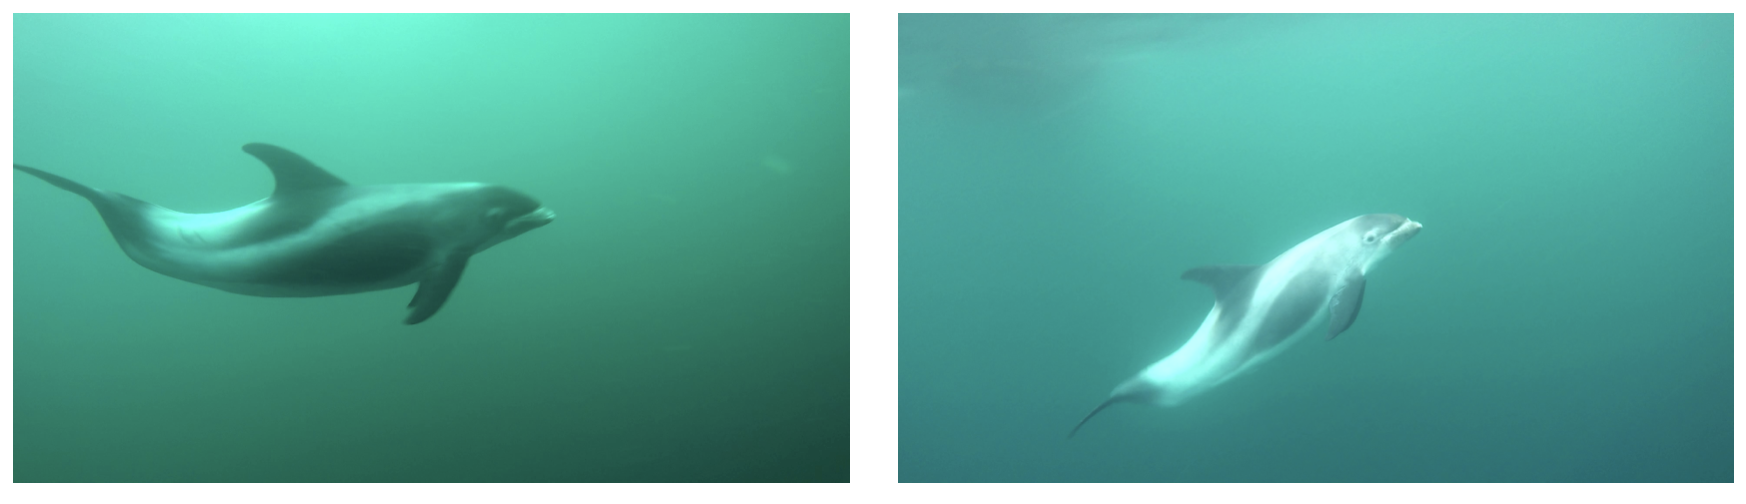
\includegraphics[scale=0.5]{Chapter4/figs/uweg.png}
	\end{center}
	\caption{Example below water images. Both images contain one mask with the following attributes: Left - \texttt{object:dolphin}, \texttt{ID:9}, \texttt{out of focus:false}. Right - \texttt{object:dolphin}, \texttt{ID:30}, \texttt{out of focus:false}.}
	\label{fig:below-water-example}
\end{figure}

\subsection{NDD20 Summary}\label{ch:NDD,sec:NDD20,sub:NDD20Summary}

%TODO: Summary of NDD20. Take from NDD20 paper? Num imgs, classes, etc.
% Link to access NDD20. Use in Kaggle competition.


% Basline experiments from NDD20 paper. - Other section


%%%%%%%%%%%%%%%%%%%
\nomenclature[z-MCZ]{MCZ}{Marine Conservation Zone}
\nomenclature[z-RIB]{RIB}{Rigid Inflatable Boat}
\nomenclature[z-NDD20]{NDD20}{Northumberland Dolphin Dataset 2020}

